\documentclass[a4paper]{article}
\usepackage{graphicx}
\usepackage{url}
\usepackage{twocolpceurws}
\usepackage{float}
% \usepackage{floatrow}
\usepackage{caption}
% \usepackage{adjustbox}
\usepackage{subcaption}
\usepackage{subfig}
\usepackage{balance}

\title{Predicting Software Quality through Network Analysis}

\author{
Giulio Concas \\ 
% Department of Electrical and Electronic Engineering 
% DIEE \footnote{\label{diee}Department of Electrical and Electronic Engineering} \\ University of Cagliari \\
% Piazza D'Armi, 09123 \\ Cagliari (Italy) \\ 
concas@diee.unica.it
\and
Michele Marchesi \\ 
% Department of Electrical and Electronic Engineering 
% DIEE \footnote{\label{diee}Department of Electrical and Electronic Engineering} \\ University of Cagliari \\
% Piazza D'Armi, 09123 \\ Cagliari (Italy) \\ 
michele@diee.unica.it
\and
Cristina Monni \\ 
% DIEE  \\ University of Cagliari \\
% Piazza D'Armi, 09123 \\ Cagliari (Italy) \\ 
% Department of Electrical and Electronic Engineering \\ University of Cagliari \\
% Piazza D'Armi, 09123 Cagliari (Italy) \\ 
cristina.monni@diee.unica.it
\and
Matteo Orr\'{u} \\ 
% DIEE \\ University of Cagliari \\
% Piazza D'Armi, 09123 \\ Cagliari (Italy) \\ 
% Department of Electrical and Electronic Engineering \\ University of Cagliari \\
% Piazza D'Armi, 09123 Cagliari (Italy) \\ 
matteo.orru@diee.unica.it
\and
Roberto Tonelli \\ 
% DIEE \\ University of Cagliari \\
% Piazza D'Armi, 09123 \\ Cagliari (Italy) \\ 
% Department of Electrical and Electronic Engineering \\ University of Cagliari \\
% Piazza D'Armi, 09123 Cagliari (Italy) \\ 
roberto.tonelli@dsf.unica.it
}

% \author{
% Mary Y. Writter \\ Publishing Dept.\\
%                 Paper City, PUB 11011 \\ mqw@pubdept.eu
% \and
% John X. Ceur \\ Science Dept.\\
%                 Online City, CEUR 99099 \\ jqq@ceur-ws.org
% \and
% Yvonne Onderzoeker \\ Research Dept.\\
%                 Science City, Sci 88088 \\ yvo@science.rdept.net
% }

\institution{Department of Electrical and Electronic Engineering (DIEE)\\ 
	     University of Cagliari \\
             Piazza D'Armi, 09123 Cagliari (Italy)}

\begin{document}
\maketitle

\begin{abstract}
We used a complex network approach to study the evolution of a large software system, 
Eclipse, with the aim of statistically characterize software defectiveness along the time.
We studied the software networks associated to several releases of the system, 
focusing our attention specifically on their community structure, modularity and clustering coefficient. 
We found that the maximum average defect density is related to two different metrics: 
the number of detected communities inside a software network
and the clustering coefficient. 
These two relationships both follow a power-law distribution which leads to a linear correlation 
between clustering coefficient and number of communities.
These results can be useful to make predictions about the evolution of software systems, 
especially with respect to their defectiveness.
\end{abstract}


\section{Introduction}
\label{sec:introduction}
% introduction to modularity

Modern software systems are large and complex products, built according to a modular structure, where 
modules (like classes in Object Oriented systems) are connected with each other 
to enable software reuse, encapsulation, information hiding, maintainability and so on. 
Software modularization is acknowledged as a good programming practice \cite{Parnas:1972, Baldwin:1999, Sanchez:1996} 
and a certain emphasis is put on the prescription that design software with low coupling and high 
cohesion would increase its quality \cite{Chidamber:1994}.  
In this work we present a study on the relationships between software systems quality and their modular structure.
Depending on the fact that software systems are inherently complex, 
%as far as the authors' knowledge, 
the best model to represent them is by retrieving their associated networks 
and the related topological 
properties \cite{Myers:2003, Subelj:2011, Wen:2008, Subelj:2014, Zimmermann:2008}.
In a software network nodes are associated to software modules (e.g. classes) and
edges are associated to connection between software modules (e.g. inheritance, collaboration relationships).
We investigated the software modular structure - and its impact in software quality - 
by studying specific network properties: community structure, modularity and clustering coefficient.
A community inside a network is a subnetwork of densely connected nodes when 
compared to nodes outside the community \cite{Girvan:2002}. 
Modularity is a function that measures how marked is a community structure 
(namely the way the nodes are arranged in communities) \cite{NG:2004}.
The clustering coefficient represents a measure of how much nodes are connected  inside a network \cite{Newman:2003}. 

% Modern Object Oriented software systems are built according to a modular structure, 
% where many interacting elementary units, like software modules, classes, objects, 
% depend on and are connected to each other, in order to optimize 
% software reuse, encapsulation, information hiding, maintainability and so on.

% the following is a repetition?
% Modularity in Software Engineering is the property of a software which is well separated
% into simpler components
%, called modules, 
% according to their functionalities and responsibilities.

% insert references (which is good) but repeat the advantages!
% Modularization has been devised as a good programming practice since the pioneer work
% of Parnas \cite{Parnas:1972}, and also more recent works \cite{Baldwin:1999, Sanchez:1996}
% explain its many advantages.

% repetition of the advantages from the first paragraph?
% The separation into almost independent components makes the
% whole system more comprehensible, enabling easy replacement of components.
% From a managerial point of view, the development time is shortened
% because developers can work on each module with little need for communication.

% \textbf{Modularity is thus acknowledged as an important feature of software systems and it is related to its quality (PLACE A REF HERE??).
% Moreover, software engineering best practices encourage developers to design software components the way they have low coupling and high cohesion.}
% % Despite the fact that modularity is acknowledged as a significant software property,  
% \textbf{Despite the fact that some metrics like ``Lack of Cohesion M???'' (LCOM) and ``Coupling Between Objects'' (CBO) \ref{Chidamber:1994} 
% return an information about the separation of software modules, by and large, we lack of a precise definition of modularity and there is no metric to characterize it.}. 
% % Moreover, in software engineering, it is widely acknowledge that a good design practice consists in keeping coupling between modules low 
% % and cohesion among them high.  
% \textbf{On the other hand, modern software systems are composed by a large number of modules, 
% among which there are an even larger number of connections, 
% that could be difficult to tackle the problem of characterize software modularity.} 
% A way to provide a measure of modularity (???) comes by approaching the study of software system by modelling them as a complex network (CITE CHINESE PAPER???)}.
% -->
% From this perspective, our study can be seen as a first attempt to provide a synthetic measure of software modularity using
% a complex network model. <---
% Modularity has been proven to be 

% In this scenario, as far as authors' knowledge, the best candidate model to represent a software system is the complex network.
% In order to perform a network analysis we need to associate to a software system 
% The size of a modern software project, as measured by the number of modules, 
% can easily reach tens of thousands of elementary units, 
% and among such modules there is an even larger number of connections, namely the
% different kind of software relationships, like inheritance, 
% composition, dependencies and others.
% As far as authors' knowledge, complex network are one of the best candidate to represent a software system
% Being the size of a modern software project, as measured by the number of modules, 
% in numbers of tens of thousands of elementary units, 
% and among such modules there is an even larger number of connections, namely the
% different kind of software relationships, like inheritance, 
% composition, dependencies and others.
% In this work we reported the results of our attempt to characterize the software quality by studying the network associated to software systems.
We studied several releases of a large software system, Eclipse, performing a longitudinal analysis 
on the relationship between community structure, clustering coefficient and software quality. 
Our aim is to figure out if the studied metrics can be used to predict software quality of future releases.
% Specifically, we focus our attention on the relationship between modular organization of software system (namely their community structure) 
% as detected by analysing network topology and the defectiveness of software modules (namely their classes) as reported in their Issue Tracking Systems (ITS).
% We performed a study on the evolution of the systems, analysing several releases of each system, to figure out if the studied metrics can be used to predict 
% quality of future releases.

This paper is organized as follows. In Section \ref{Methodology} we illustrate the methodology. In Section \ref{Results}, we present and discuss some of our results 
and finally, in Section \ref{Conclusions}, we report our conclusions.
% explain how we built the analysed networks and retrieved
% the metrics we are interested in. 
% Our findings, reported in Section \ref{sec:results}, are multifaceted and span different aspects of the application 
% of community detection to software systems. They provide the answers to the Research Questions, which are discussed in detail in Section
% \ref{sec:discussion}. We end with our Conclusions in Section \ref{sec:conclusions}.
% 
% However, a great degree of modularity does not only bring benefits to system design.
% Sometimes, if modules are very specific, the cost of making interfaces can be high \cite{Schilling:2000}. 
% It can also be difficult to understand the interaction between modules or to integrate them,
% or it can affect design creativity \cite{Schilling:2000, Arnheiter:2006}. 
% Sometimes, high modularity can affect the total system performance \cite{Arnheiter:2006}. 

% Such modularity, along with interconnections among modules, the large number of modules, 
% the complexity of their interconnections, are all signatures of a structure
% which has been demonstrated to belong to the class of complex networks \cite{Myers:2003}. 
% Software systems exhibit scale-free and small-world properties, like those identified in other technological, 
% sociological, and biological systems \cite{Jenkins:2007}, and it is thus sensible to study them using techniques and instruments adopted for analyzing complex networks. 
% 
% One of the main issues when investigating complex networks properties 
% is the problem of determining their community structure, if any. 
% This issue, born in the discipline  
% of social analysis, has become increasingly interesting in the field of 
% complex networks, where many systems 
% from very different fields have been 
% found to 
% display a clear community structure \cite{Subelj:2011, Clauset:2004, Fortunato:2010, NFast:2004, NG:2004}.
% 
% The problem resides in finding the optimal division of a network in "communities" that is, 
% set of nodes tightly connected, 
% according to some measure, and characterizing the community structure by
% measuring different metrics for the obtained partition. 
% The most common approach is the optimization of a 
% \textit {modularity function}
% over the possible divisions of a network.
% The organization of networks in communities, 
% with many edges among vertices of the same cluster and 
% comparatively few edges joining vertices of different clusters
% can reveal fairly independent parts of the network, each playing its own role, 
% and can be of great importance in the field of software systems. 
% In this work we use community detection in software networks, 
% with the aim of detecting community structures in software systems 
% and of using community metrics to analyze and characterize software quality. 
% 
% In the literature there are other attempts to relate software quality to other
% network metrics, such as degree distribution \cite{Turnu:2012}, fan-in and fan-out
% \cite{Murgia:2012} or more generally, to software metrics \cite{Concas:2012a}. 
% Some works focus more on fault prediction, for example via machine-learning algorithms \cite{Catal:2009}.
% Here we focus in particular on community metrics, which 
% are more familiar in the social network context. 
% These metrics can be related to some properties of software systems, such as defectiveness or modularity.
% 

% 
% In this work we address another kind of modularity, defined in complex networks, and apply it to
% software networks.
% This modularity, denoted by $Q$, depends on the topology of the network, and in principle it
% is not related to the functionality of the system underlying the network.
% However, we aim at understanding if the modularity retrieved by specific algorithms for a software network could be related
% to the modularity defined in software design.
% Just as communities in a software network, modules are connected to one another, and often modules coincide
% with communities, meaning that the functional design of a software system and 
% the topological structure of the corresponding network are closely related. 
% 
% Moreover, in software engineering, a good design practice consists in keeping coupling low 
% and cohesion high. 
% In the corresponding software network, where the simpler components are the communities,
% the number of edges between communities can give a measure of inter-community relationships, while the number of edges 
% inside each community could be linked to cohesion.
% The modularity $Q$ gives an indication of the ratio between the number of intra- and inter-community
% edges. When $Q$ is maximal, communities are well separated, which would mean there is high cohesion and 
% low coupling, if communities and modules are somehow equivalent. So high modularity values could indicate that
% the analyzed software system has been designed using good programming practice.
% However, this is not always the case. Sometimes modules and communities do not match, and a high degree of modularity
% in the software Engineering sense, does not coincide with a high value of modularity $Q$ for software networks.
% It is thus interesting to investigate if the two different modularities can be put in relationship with each other,
% since they both can give indications on software quality. Moreover, while modularity in software design is
% a property at design level, before the whole system is realized,
% network modularity $Q$ is known only after the system has been designed and realized.
% If these two metrics are related, it could be possible
% to understand how design decisions would affect system topology and functionalities.
% 

% 
% We analyzed 
% several hundreds of sub-projects from different releases of Eclipse and Netbeans,
% two large Open Source Object Oriented (OO) software systems written in Java. 
% These are two popular Integrated Development Environments (IDEs).
% These systems are composed by many almost independent sub-systems that could be analyzed separately.
% We analyzed different releases along time, so we were able
% to consider the evolution of the properties under study.
% The analyzed releases are Eclipse 2.1, 3.0, 3.1, 3.2, 3.3, 
% and Netbeans 3.2, 3.2.1, 3.3.0, 3.4, 4.0, 6.0.1.
% 
% 
% This work improves a recent preliminary research 
% of the authors on the same subject \cite{Concas:2013}, and examines for the first time,  
% to authors' knowledge, the relationship among different software
% properties and metrics related to community 
% structure and system defectiveness for large software networks. 
% 
% To formulate the research questions we rely on the Goal Question Metrics method of Basili et al. \cite{Basili:1994}.
% According to this approach, we first identify a \textit{goal}, then define some \textit{research questions} and 
% eventually choose some \textit{metrics} to associate to each question.
% The goal is composed by the \textit{purpose}, the \textit{perspective} and the \textit{environment}.
% In this work our aim is to investigate software systems (the \textit{object} of our analysis) to figure out if 
% there are relationships among some of the properties of the related software network and software quality. 
% Here we show that it is possible provide a statistical characterization of the defectiveness of the analyzed software systems in future releases. 
% 
% It is widely accepted that an important marker of a software system quality is the presence (or the absence) of software defects.
% As a consequence, the perspective of our research is to understand if software defects have a significant
% relationship with software network topology, and how to use this information to predict the quality of future releases.
% These predictions can be considered also from the viewpoint of a software developer or of a team leader.
% The model for software quality is the number of defect per class, called defect density, while
% the reference model for software systems is the software network.
% Finally, the environment is represented by the studied releases of Eclipse and NetBeans.
% The properties of software systems we are interested in are their community structure and the related metrics: modularity, number of communities
% and clustering coefficient.
% This leads us to investigate the following research questions:
% 
%  \begin{enumerate}
%  
%   \item  Is defectiveness related to network modularity?
%   \item  Is defectiveness related to the number of communities?
%   \item  Is defectiveness related to network's clustering coefficient?
%  
%  \end{enumerate}
% 

\section{Related Work}
\label{sec:related work}

\textbf{DAL PRIMO WETSOM}

%One of the key concepts of OO paradigm is the class, which provides 
%the definition of objects, single units where operative code resides, 
%interacting with other objects in the system by the exchange of messages. 
%The exchange of messages at run time is determined 
%at the source code level by the relationships among the 
%different classes, 
%such as inheritance, composition, aggregation,
%association, dependence and so on. 
Many software systems have reached such a huge dimension that it looks sensible to treat them as 
complex networks \cite{Focardi:2001}, \cite{Myers:2003}, \cite{Turnu:2011}. 
In particular, software networks made of thousands of nodes 
show properties typical of complex networks \cite{Barabasi:2000}, like 
a power law distribution of the node degree, scale free properties \cite{Song:2005}, fractal and self-similar features
\cite{Turnu:2012}, the small world property, power law scaling for 
bug distribution \cite{TSE:2011}, for refactored classes \cite{CSMR:2012}, 
and so on. 
In the field of software, class diagrams \cite{Valverde:2002, Valverde:2003}, 
the software 
collaboration graph \cite{Myers:2003}, the package dependencies networks \cite{Challet:2004}, 
have been found to belong to the complex networks category.
In our case networks nodes are Netbeans classes, and network edges 
are class dependencies.
%\input{related_2}
%Software systems are designed to be highly evolvable \cite{Myers:2003}, in order to be modified to meet new requirements along 
%the time and this evolvability is acquired by decoupling the different subsystems, to
%prevent the risk of side-effects when introducing new functionalities.
%Several authors applied network analysis to the study of software complex systems to gain major knowledge on the 
%structure and behavior of complex systems and also to gather significative information in order to better address the issue of
%developers' effort at each stage of software development. 
%\cite{Wen:2007, Li:2008}.
%[16, 27, 32, 34]. 
In \cite{Wen:2007} it has been shown that the knowledge of scale-free properties of software networks
could be useful to reduce the time devoted to maintenance. 
\v{S}ubelj and Bajek, after analyzing different Java softwares using a community detection algorithm, find that the software systems analyzed 
exhibit a significant community structure that doesn't match the packages structure imposed by the designer \cite{Subelj:2011}. 
\\
The community structure is 
one of the properties that recently grabbed researchers' attention. 
Inside a network a community is a set of vertices between which there is a high density of connections. 
On the contrary between the communities connections are more sparse. The community structure of a network is its 
division in subgroups or communities \cite{NG:2004}.
Elements belonging to the same community are more likely to share the same behavior or properties, or represent a functional unit. 
This leads to many concrete applications of community detection in different fields (from marketing research to software development). 
%Modern software systems are structured in subsystems, generally organized in a hierarchical manner, 
%where small units cooperate with each other to carry out 
%complex tasks through collaboration and information interchange. 
%For this reason, the community structure analysis applied to software networks can give some insights on the structure
%and functionalities of the software.
%Software engineering practices emphasize the decomposition of complex tasks in smaller ones, to encourage code reuse 
%and agile development \cite{IJSEKE:2012}. 
%Specifically, studying the community structure of a complex network can help to understand how a software system is 
%organized in functional modules. 
%Many authors analyzed software systems developed in different programming languages and styles and find evidences that 
%they show scale-free properties (see, for example, \cite{Wen:2007}). 
%[18, 27, 35]. 
%Others \cite{Li:2008}, after having analyzed different java softwares using a community detection algorithm, find that the software systems analyzed 
%exhibit a significant community structure that doesn't match the packages structure imposed by the designer. 
\\
Community detection is traditionally addressed using techniques like hierarchical clustering and partitional clustering 
\cite{Fortunato:2010} and it faces different problems. One of the most important is finding algorithms that allow network
scalability up to different orders of magnitude 
(from thousands to millions of vertices) to be analyzed in a reasonable amount of time. 
\\
Newman \textit{et al.} proposed several algorithms for community detection
\cite{NG:2004, NFast:2004, Clauset:2004} using different approaches and dealing with the problem of the computational burden. 
Moreover, in \cite{NG:2004} Newman and Girvan introduced a quality function called \textit{modularity}, 
to evaluate how good is a network partition in communities. 
%si parla della modularità, conviene introdurre qui la definizione
In our case study, the analysis of the community structure of the software 
network can help to understand how the software system is organized 
in functional modules. 
\\
In this paper we analyze the community structure 
of the 56 Netbeans subprojects and the community 
properties of each subproject in order to recover information about 
the software structure and quality. We compute four  
typical metrics for the communities, namely the modularity, 
the clustering coefficient, the mean degree and the average path length, 
and compare these metrics to data extracted from the 
software subprojects, such as the number of defects or the 
number of packages. 
To accomplish this comparison we use the research questions approach, 
formulating three questions: 
\begin{itemize}

\item \textbf{RQ1}: \textit{Are there correlations between the 
community structure and software defectiveness?} 

\item  \textbf{RQ2}: \textit{Are there correlations between the community 
metrics and software defectiveness?}

\item  \textbf{RQ3}: \textit{Do the software networks analyzed present a community structure that matches the package
structure devised by developers? 
%If this circumstance occurs, to which extent this matching is present? 
%Is there a quantitative measure of the matching or mismatching?
}
\end{itemize}
The answers to these research questions will be discussed after the analysis 
of the results. 



\section{Methodology}
\label{Methodology}

In this work we aim at analysing the structure of a software system using its associated software network.
In order to build the associated software network we parsed software's source code, retrieved from the corresponding Software Control Managers (SCM). 
During this procedure, we associate network nodes to classes and network edges 
to the various relationships between classes (inheritance, composition, etc.). 
We consider the number of defects (bugs) as a main indicator of software quality. 
To exploit this we collected data about the bugs of a software system by 
mining its Bug Tracking Systems (BTS). 
Bugzilla is the BTS adopted by Eclipse, where defects are tagged with a unique ID number.
Usually an entry in BTS is called with the common term 'Issue', and there is usually 
no information about classes associated to defects.
Usually all the maintenance operations on software systems are reported on Software Configuration Management
(SCM) systems like Concurrent Version Systems\footnote{CVS, http://www.nongnu.org/cvs/.},
Git and Subversion. 
However, it is not possible to distinguish between bug fixings or
other actions such as enhancements, since all maintenance operations on software systems are recorded as "commit 
operations".
To obtain a correct mapping between Issue(s) and the related 
Java files (CUs), 
we analyzed the SCM log messages, to identify commits associated to
maintenance operations where Issues are fixed. 
If a maintenance operation is done on a file to address a defect, 
we consider the CU as affected by that defect. \\
We first analyzed the text of commit messages, looking for Issue-IDs.
Unfortunately, every positive integer number is a potential Issue-ID. However, sometimes
numbers that refer to maintenance operations are not related to Issue-ID resolution, but, for example,
to branching, data, number of release, copyright updating, and so on. 
To avoid wrong mappings between Issue-IDs and CUs, we applied the following rules:
\begin{itemize}
\item In each release, a CU can be affected only by Issues which are referred to in the BTS as belonging to the same release.
\item All IDs not filtered out are considered Issues and associated to the addition or modification of one or more CUs, as reported in the commit logs. 
\item When assigning  defects to classes in the corresponding CUs, since there were 
few CUs containing more than one class, we decided to assign all the defects to the biggest 
class of those CUs.
\end{itemize}

This method might not completely address the problems 
of the mapping between defects and CUs \cite{Ayari:2007}. 
In any case we checked manually 10$\%$ of randomly chosen CU-defect(s) associations for intermediate releases
and every CU-defect association for 
3 sub-projects without finding any error. A bias may still remain 
due to lack of information on SCM \cite{Ayari:2007}. 
The subset of Issues satisfying the conditions as in Eaddy et al. is the Bug-metric \cite{Eaddy:2008}. 
Of course there are chances for wrong assignments to happen for 
some classes, but since the average number of defects for class is very low,
the number of wrong assignments in the entire system, considering also 
CUs with one class, is very limited. 
\\
At the end of this process we obtained a network where 
to each node is associated the number of bugs of the corresponding class. 

We collected the source code and analysed 5 releases of Eclipse, whose main feature are 
presented in Table \ref{tab:Eclipse}. 

\begin{table}[h]
\begin{center}
\begin{tabular}{|l|c|c|c|c|c|}
\hline 
\textbf{Release} &\textbf{  2.1} & \textbf{ 3.0} &  \textbf{3.1 }&  \textbf{3.2} &  \textbf{3.3
} \\
Size & 8257 & 11406 & 13413 & 16013 & 17517 \\
 
Sub-Projects n.& 49 & 66 & 70 & 86 & 104 \\ 

N. of defects & 47788 & 59804 & 69900 & 80149 & 95337  \\ \hline


\end{tabular}
\end{center}
\caption{Main features of the analysed releases of Eclipse (EC): size (number of classes), 
number of sub-projects (sub-networks), and total number of defects.}
\label{tab:Eclipse}

\end{table}

Each release is structured in almost independent sub-projects. The total number 
of sub-projects analysed amounts at 375, with more than 60000 nodes (classes) 
and more than 350000 defects.% 170623

We detected the associated community structure using the algorithm devised by 
Clauset et al. \cite{Clauset:2004}. 
This is an agglomerative clustering algorithm that performs a greedy optimization 
of the Modularity (Q) \cite{Newman:2003}. 
At the end we retrieved the number of communities in which the network is structured, 
the corresponding value Q of the modularity, and the nodes associated to each community. 
We performed the computation of the clustering coefficient using the implementation 
included in the IGraph software 
\cite{igraph}. 
To study the system's evolution we used the following approach. We first 
carried out the analysis for each release, and then we assembled together 
different releases, according to a temporal evolution. 
More precisely, for the 5 releases of our dataset, we
studied the evolution of the system by cumulating the first and 
the second releases in a single set, then adding the third release 
to this first set to obtain a second set and so on. 
This way we were able to make predictions about the next release 
starting from those cumulated in the previous assembly.



\section{Results}
\label{Results}

% \subsection{Defect Density Prediction}
Figures \ref{fig:abn-noc} and \ref{fig:cc-noc} show the distributions of the average bugs number 
(ABN, Fig. \ref{fig:abn-noc}) 
and of clustering coefficient (CC, Fig. \ref{fig:cc-noc}) with respect to the number of communities (NOC) 
for all the sub-projects of all the releases. 
Although the scatterplots for the relationship between NOC % number of communities 
and other metrics are sparse, the reported scatterplots show the existence
of a power-law-like relationship between the maximum values of the mentioned metrics. 
This led us to hypothesize a linear relationship between the maximum values of 
CC and the ABN. % average bug number. If this is the case the CC can be used to predict the maximum ABN % average number of defects 
% in a future release, 
% having cumulated the data belonging to the previous releases.
In Tab. \ref{tab:log-log-cc-noc}, on the left, the power law exponents, 
the correlation coefficient, the $\chi^2$ and the degrees of freedom (\textit{dof}) for the best fitting in log-log scale are reported. 
They refer to different ``cumulated''
releases for the relationship between CC and NOC. % clustering coefficient and the number of communities. 
Table \ref{tab:log-log-cc-noc} shows how the power laws parameters do not change significantly from one cumulated release to another. 
This suggests the existence of a progressively more stable behaviour during 
software evolution, where the fitting with a power law becomes 
more accurate and tends to a fixed value as new releases are added 
in the cumulated dataset.
The same considerations can be applied to the relationship between maximum ABN 
and NOC. % average bugs number and number of communities.
% stabilize around a fixed value
% Namely, with the addition of more releases, .
The scatterplot portraied in Fig. 2 % \ref{cumulated_bug_cc_EC} 
shows the relationship between the maximum defect density versus the maximum clustering coefficient, 
for all the cumulated releases, along with the best fitting straight line.
We investigated if, starting with a dataset of $N$ releases, the best fitting curve for the cumulated $N -1$ releases 
could also be a good fit for the $Nth$ release.
In order to measure the forecast accuracy we adopted a $\chi^2$ test.
Table \ref{tab:max_abn-vs-maxcc} reports the results of the best fitting for the relationship between CC and ABN showing that the linear correlation is not very high. 
Nonetheless, the $\chi^2$ test returns an high level of significance.
Table 2 % \ref{prevision_test} 
reports the results of the analysis on the forecast for software quality. 
We computed the ratio between the $\chi^2$ and the degrees of freedom. 
% The reported $\chi^2$ values are close to 1, meaning that for the given degrees of freedom the fits are good.
According to the results reported on Table \ref{tab:log-log-cc-noc}, on the right, the 
$\chi^2$ values are close to 1, meaning that for the given degrees of 
freedom the fits are good.

\begin{figure*}
        \centering
        \begin{subfigure}%[b]
        {0.3\textwidth}
                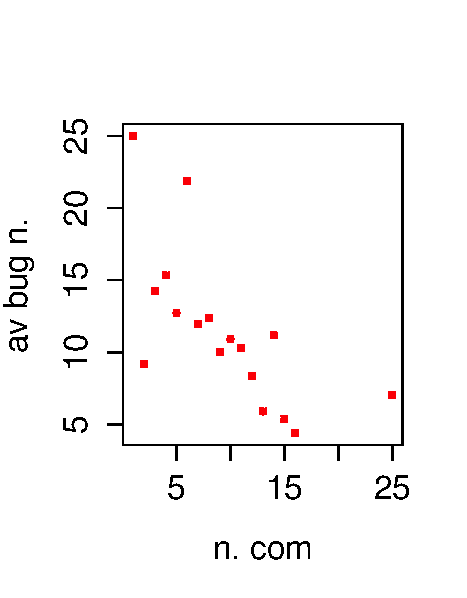
\includegraphics[width=\textwidth]{figure/EC_BUG_power_law-eps-converted-to.pdf}
                \caption{Average Bug Number vs. Number of Communities}
                \label{fig:abn-noc}
        \end{subfigure}%
        ~ %add desired spacing between images, e. g. ~, \quad, \qquad, \hfill etc.
          %(or a blank line to force the subfigure onto a new line)
        \begin{subfigure}%[b]
        {0.3\textwidth}
                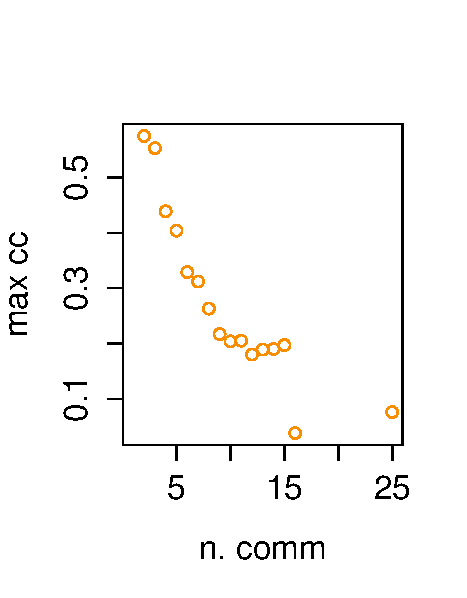
\includegraphics[width=\textwidth]{figure/EC_CC_power_law-eps-converted-to.pdf}
                \caption{Clustering Coefficient vs. Number of Communities}
                \label{fig:cc-noc}
        \end{subfigure}

        \caption{Scatterplot of the relationships between the studied metrics.}
        \label{fig:scatterplot-abn-cc-noc}
\end{figure*}

\begin{table}%[htbp]
\centering
\begin{tabular}{|c|c|c|c|c|c|}
\hline
\textbf{Releases} & $\alpha$ & $r$ & $\chi^2$ & $dof$  \\
      2.1 - 3-0   & -1.010  & -0.654 &  0.075 & 16 	 \\
      2.1 - 3.1   & - 0.917 & -0.667 &  0.057 & 17 	 \\ 
      2.1 - 3.2   & -0.977  & -0.715 &  0.087 & 20	 \\ 
      2.1 - 3.3   & -0.986  & -0.712 &  0.119 & 21	 \\
\hline
\end{tabular}
\caption{Results on the power law between maximum Clustering Coefficient vs Number of communities for Eclipse: exponent $\alpha$, 
correlation coefficient ($r$), value of Chi Squared ($\chi^2$ ) and number of degrees of freedom ($dof$). 
}
\label{tab:log-log-cc-noc}
\end{table}
\begin{table}
\centering
          \begin{tabular}{|c|c|c|c|c|c|}
	\hline
	\textbf{Eclipse} & max ADD vs NOC & max CC vs NOC \\ 	
		     dof & 13 & 13 \\
		    $\chi^2$ / dof & 0.361 & 1.005 \\ \hline
	      \end{tabular}
\caption{Fit data for the power laws between the maximum average defect density (max ADD) versus the number of communities
and maximum clustering coefficient (max CC) versus the number of communities: correlation coefficient ($r$), 
      normalized Chi squared ($\chi^2$ ), and number of degrees of freedom ($dof$).}
\label{tab:lin-fit-cc-and-add}
\end{table}

\begin{figure*}[!htbp]
     \centering
    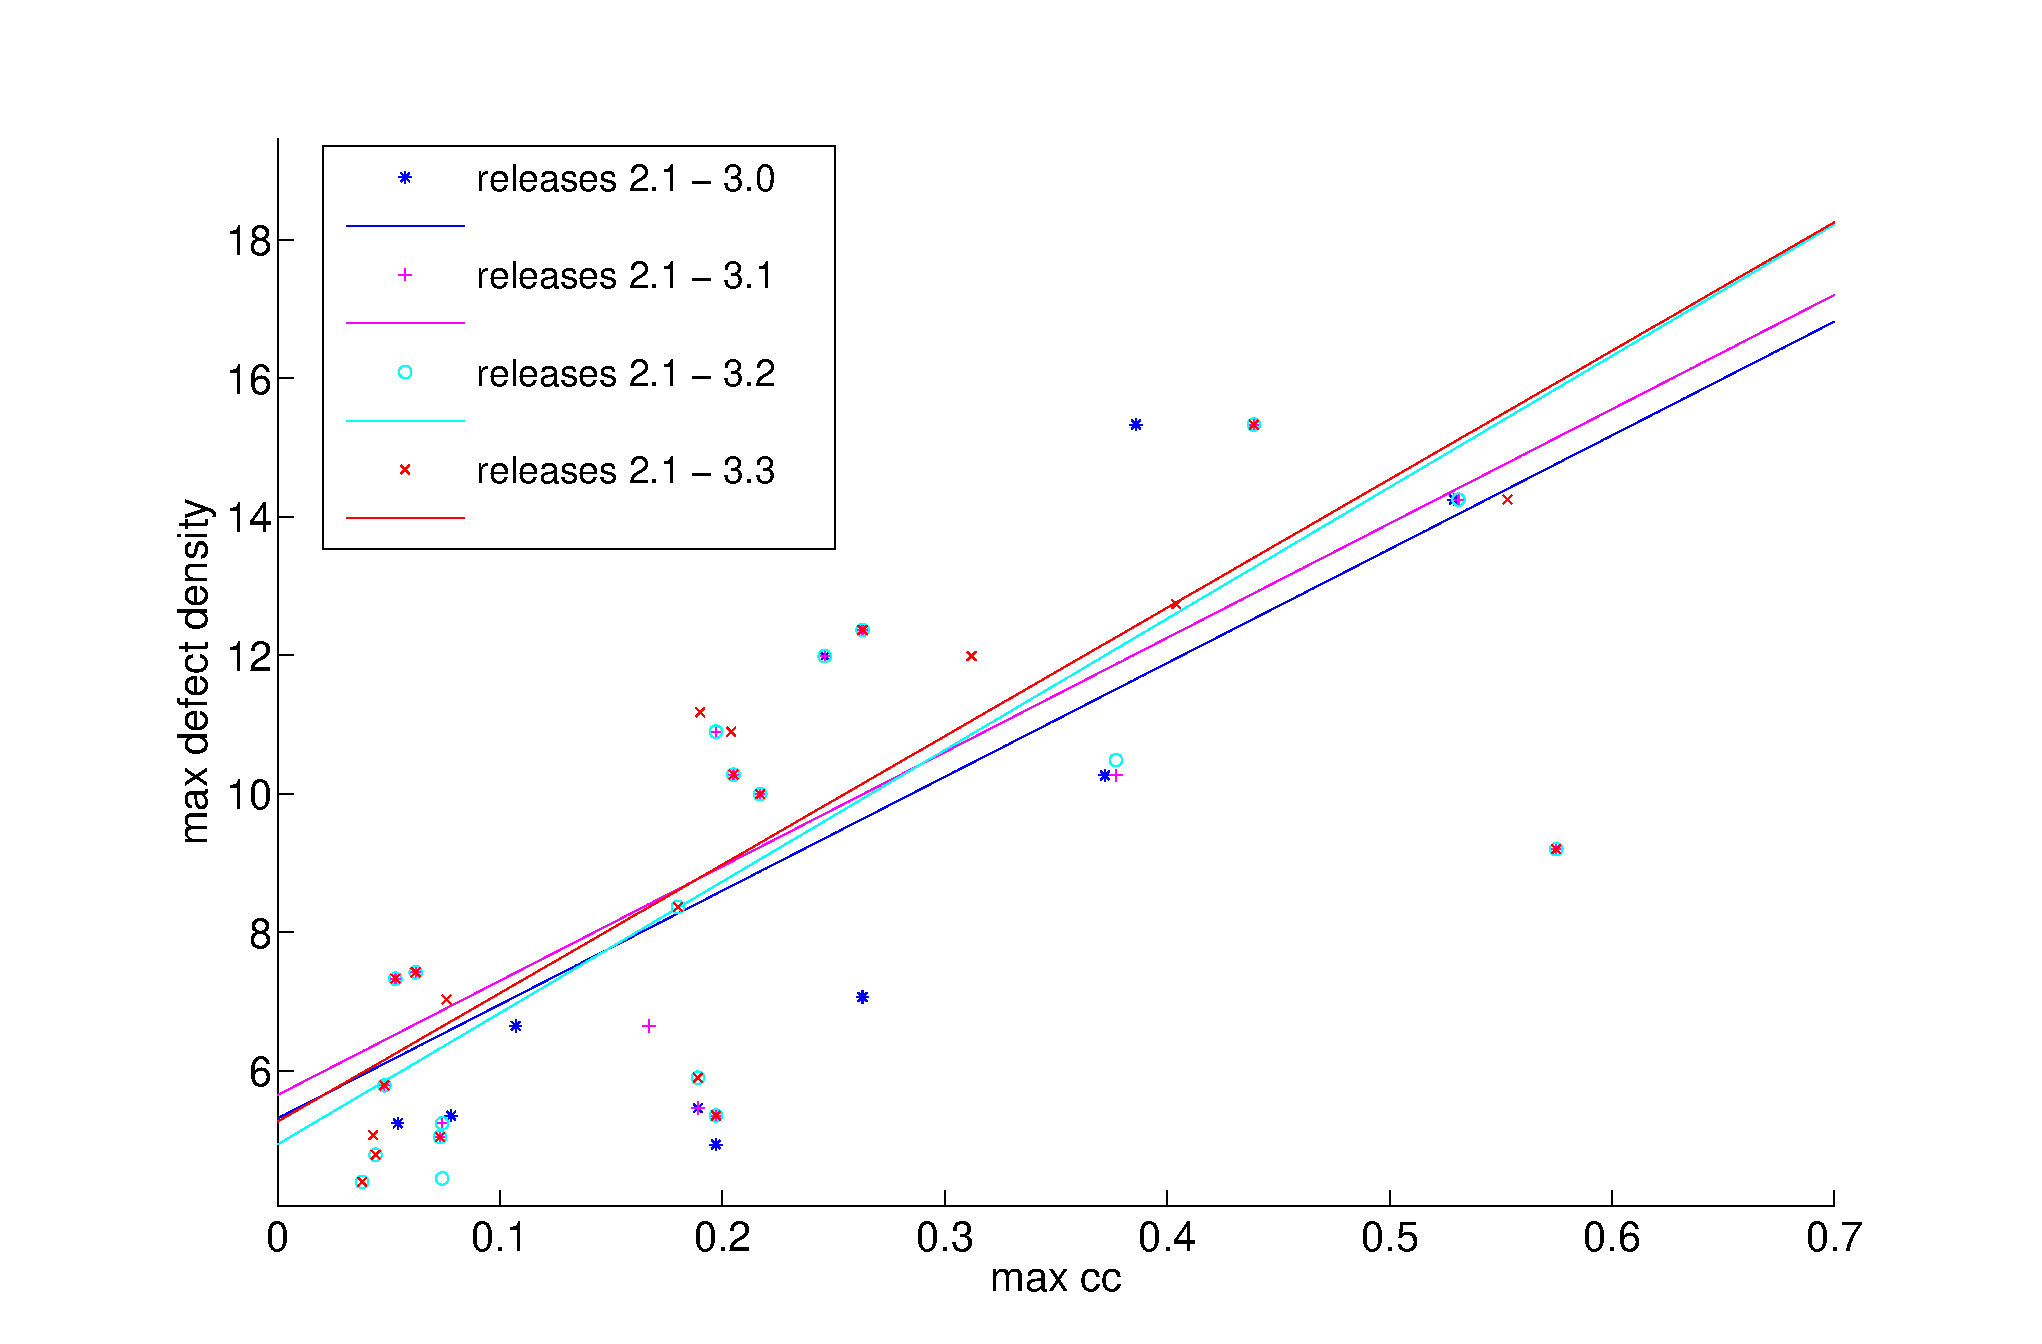
\includegraphics[width=\textwidth]{figure/nuovefig/cumulated_bug_cc_EC.eps}
    \label{cumulated_bug_cc_EC}
    \caption{Cumulated plots and fitting lines for the maximum defect density vs maximum clustering coefficient.}
\end{figure*}

    \begin{table}
    \centering
      \begin{tabular}{|l|c|c|c|}
      \hline
      \textbf{Releases} & $r$ & $\chi^2$ & $dof$  \\
      2.1 - 3-0 & 0.565 & 0.633 & 16  \\
      2.1 - 3.1 & 0.576 & 0.651  & 17  \\
      2.1 - 3.2 & 0.677 & 0.523 & 20 \\ 
      2.1 - 3.3 & 0.687 & 0.547 & 21 \\
      \hline
      \end{tabular}
       \caption{Fit data for the maximum defect density vs maximum clustering coefficient: correlation coefficient ($r$), 
      normalized Chi squared ($\chi^2$ ), and number of degrees of freedom ($dof$).}
\label{tab:max_abn-vs-maxcc}      
\end{table}
  


\section{Conclusions}
\label{Conclusions}
In this work we presented a longitudinal analysis on the evolution of a large software system with a focus on software defectiveness.
Through a complex network approach we were able to study the structure of 
the system by retrieving the community structure of the associated 
network. After retrieving the number of defects associated to the 
software network classes, we performed a topological analysis detecting the 
community structure. 
We found a power law relationship between the maximum values of the clustering coefficient, the average bug number and the division in communities of the software network. This lead to a linear relationship between the maximum values of clustering coefficient and of average bug number.
We show that such relationship can in principle be used as a predictor for the maximum value of the average bug number in future releases. 


\bibliographystyle{alpha} 
\balance
\bibliography{sigproc, reftest, ese_bibliography, sattose}


% \section{General Formatting Instructions}
% 
% The format is in one column. The left margin is .9 inches (5.5 picas). Use 10 point type,
% with a vertical spacing of 11 points. Times Roman is the preferred
% typeface throughout.
% 
% Paper title is 16 point, Caps/lowercase, bold, centered. Subsequent
% pages should start at 1 inch (6 picas) from the top of the page.
% 
% Authors names are centered, initial caps; co-authors names, if used, are
% flush left and flush right.
% 
% Paragraphs are indented by 1 pica with no space between paragraphs.
% 
% \section{First Level Heading}
% 
% First level headings are all flush left, initial caps, bold and in point
% size 12. One line space before the first level heading and $1/2$ line
% space after the first level heading.
% 
% \subsection{Second Level Heading}
% 
% Second level headings must be flush left, initial caps, bold and in point
% size 10. One line space before the second level heading and $1/2$ line
% space after the second level heading.
% 
% \subsubsection{Third Level Heading}
% 
% Third level headings must be flush left, initial caps and bold.
% One line space before the third level heading and $1/2$ line
% space after the third level heading.
% 
% \paragraph{Fourth Level Heading}
% 
% Fourth level headings must be flush left, initial caps and roman type.
% One line space before the fourth level heading and $1/2$ line
% space after the fourth level heading.
% 
% \subsection{Citations In Text}
% 
% Citations within the text should indicate the author's last name and
% year\cite{Knuth-vol3}. Reference style\cite{Comer-btree}
% should follow the style that you are used to using, as long as the
% citation style is consistent.
% 
% \subsubsection{Footnotes}
% 
% Indicate footnotes with a number\footnote{This is a sample footnote} in
% the text. Place the footnotes at the bottom of the page they appear on.
% Precede the footnote with a vertical rule of 2 inches (12 picas).
% 
% \subsubsection{Figures}
% 
% All artwork must be centered, neat, clean and legible. Do not use pencil
% or hand-drawn artwork. Figure number and caption always appear after the
% the figure. Place one line space before the figure, one line space
% before the figure caption and one line space after the figure caption.
% The figure caption is initial caps and each figure is numbered
% consecutively.
% 
% Make sure that the figure caption does not get separated from the
% figure. Leave extra white space at the bottom of the page to avoid
% splitting the figure and figure caption.
% 
% Figure \ref{fig1} shows how to include a figure as encapsulated postscript.
% The source of the figure is in file {\tt fig1.eps}.
% 
% \begin{figure}[ht]
% \begin{center}
% %\includegraphics[height=4cm]{fig1}
% \caption{Sample EPS figure }
% \label{fig1}
% \end{center}
% \end{figure}
% 
% Below is another figure using LaTeX commands.
% 
% 
% \begin{figure}[ht]
% \begin{center}
% \setlength{\unitlength}{1pt}
% \footnotesize
% \begin{picture}(160,80)
%         \put(0,0){\framebox(160,80)[]{}}
%         \put(10,35){\framebox(80,40){}}
%         \put(100,20){\framebox(40,20){}}
%         \put(70,10){\framebox(20,10){}}
%         \put(20,5){\framebox(10,5){}}
% \end{picture}
% \caption{Sample Figure Caption}
% \end{center}
% \end{figure}
% 
% \subsubsection{Tables}
% 
% All tables must be centered, neat, clean and legible. Do not use pencil
% or hand-drawn tables. Table number and title always appear before the
% table.
% 
% One line space before the table title, one line space after the table
% title and one line space after the table. The table title must be
% initial caps and each table numbered consecutively.
% 
% \begin{table}[ht]
% \begin{center}
% \caption{Sample Table}
% 
% \bigskip
% 
% \begin{tabular}{|l|l|r|}
% \hline
% A & B & 1\\ \hline
% C & D & 2\\
% E & F & 3\\ \hline
% \end{tabular}
% \end{center}
% \end{table}
% 
% 
% \subsubsection{Handling References}
% 
% Use a first level heading for the references. References follow the
% acknowledgements.
% 
% 
% \subsubsection{Acknowledgements}
% 
% Use a third level heading for the acknowledgements. All acknowledgements
% go at the end of the paper.
% 
% 
% 
% 
% %\bibliographystyle{alpha} 
% %\bibliography{samplebib}
% %inline the .bbl file directly for mailing to authors.
% 
% \begin{thebibliography}{Com79}
% 
% \bibitem[Com79]{Comer-btree}
% D.~Comer.
% \newblock The ubiquitous b-tree.
% \newblock {\em Computing Surveys}, 11(2):121--137, June 1979.
% 
% \bibitem[Knu73]{Knuth-vol3}
% D.~E. Knuth.
% \newblock {\em The Art of Computer Programming -- Volume 3 / Sorting and
%   Searching}.
% \newblock Addison-Wesley, 1973.
% 
% \end{thebibliography}

\end{document}


